%
% $RCSfile: inner_structure.tex,v $
%
% Copyright (C) 2002-2008. Christian Heller.
%
% Permission is granted to copy, distribute and/or modify this document
% under the terms of the GNU Free Documentation License, Version 1.1 or
% any later version published by the Free Software Foundation; with no
% Invariant Sections, with no Front-Cover Texts and with no Back-Cover
% Texts. A copy of the license is included in the section entitled
% "GNU Free Documentation License".
%
% http://www.cybop.net
% - Cybernetics Oriented Programming -
%
% http://www.resmedicinae.org
% - Information in Medicine -
%
% Version: $Revision: 1.1 $ $Date: 2008-08-19 20:41:07 $ $Author: christian $
% Authors: Christian Heller <christian.heller@tuxtax.de>
%

\subsection{Inner Structure}
\label{inner_structure_heading}
\index{CYBOI Knowledge Container}
\index{CYBOI Signal Checker}
\index{Neumann Model of a Computing Machine}

To what concerns its inner architecture, there are two basic structures
underlying CYBOI:

\begin{enumerate}
    \item \emph{Knowledge Container:} An array-based structure usable for
        storing static knowledge in form of primitive- and compound models, and
        capable of representing a map, collection, list and tree
    \item \emph{Signal Checker:} A loop-based structure usable for dynamically
        reading signals from a queue, and capable of processing them after
        their priority, in a special handler
\end{enumerate}

All modules, into which CYBOI is subdivided, are built around these two core
structures. Having read chapter \ref{state_and_logic_heading} demonstrating the
existence of state- and logic knowledge, one might argue that there should be
two knowledge containers, one for each kind. But because knowledge models may
be placed not only in space or time, but possibly other dimensions, too (like
mass, for the weights in an artificial neural network), the prototype emerging
from this work stores state- and logic-, as well as any other models in one and
the same knowledge tree.

Not unlike John von Neumann's model of a computing machine \cite{selflinux},
which distinguishes \emph{Memory}, \emph{Control Unit},
\emph{Arithmetic Logic Unit} (ALU) and \emph{Input/ Output} (i/o), CYBOI's
modules are grouped into four architectural parts, as illustrated in figure
\ref{architecture_figure}. These have the following functionality:

\begin{itemize}
    \item \emph{Memoriser:} data creation, -destruction and -access (after
        Neumann, it contains not only data, but also the operations that are
        applied to them)
    \item \emph{Controller:} lifecycle management, signal handling, i/o filters
    \item \emph{Applicator:} operation application (comparison, logic,
        arithmetic and more)
    \item \emph{Globals:} basic constants and variables, as well as a logger
\end{itemize}

\begin{figure}[ht]
    \begin{center}
        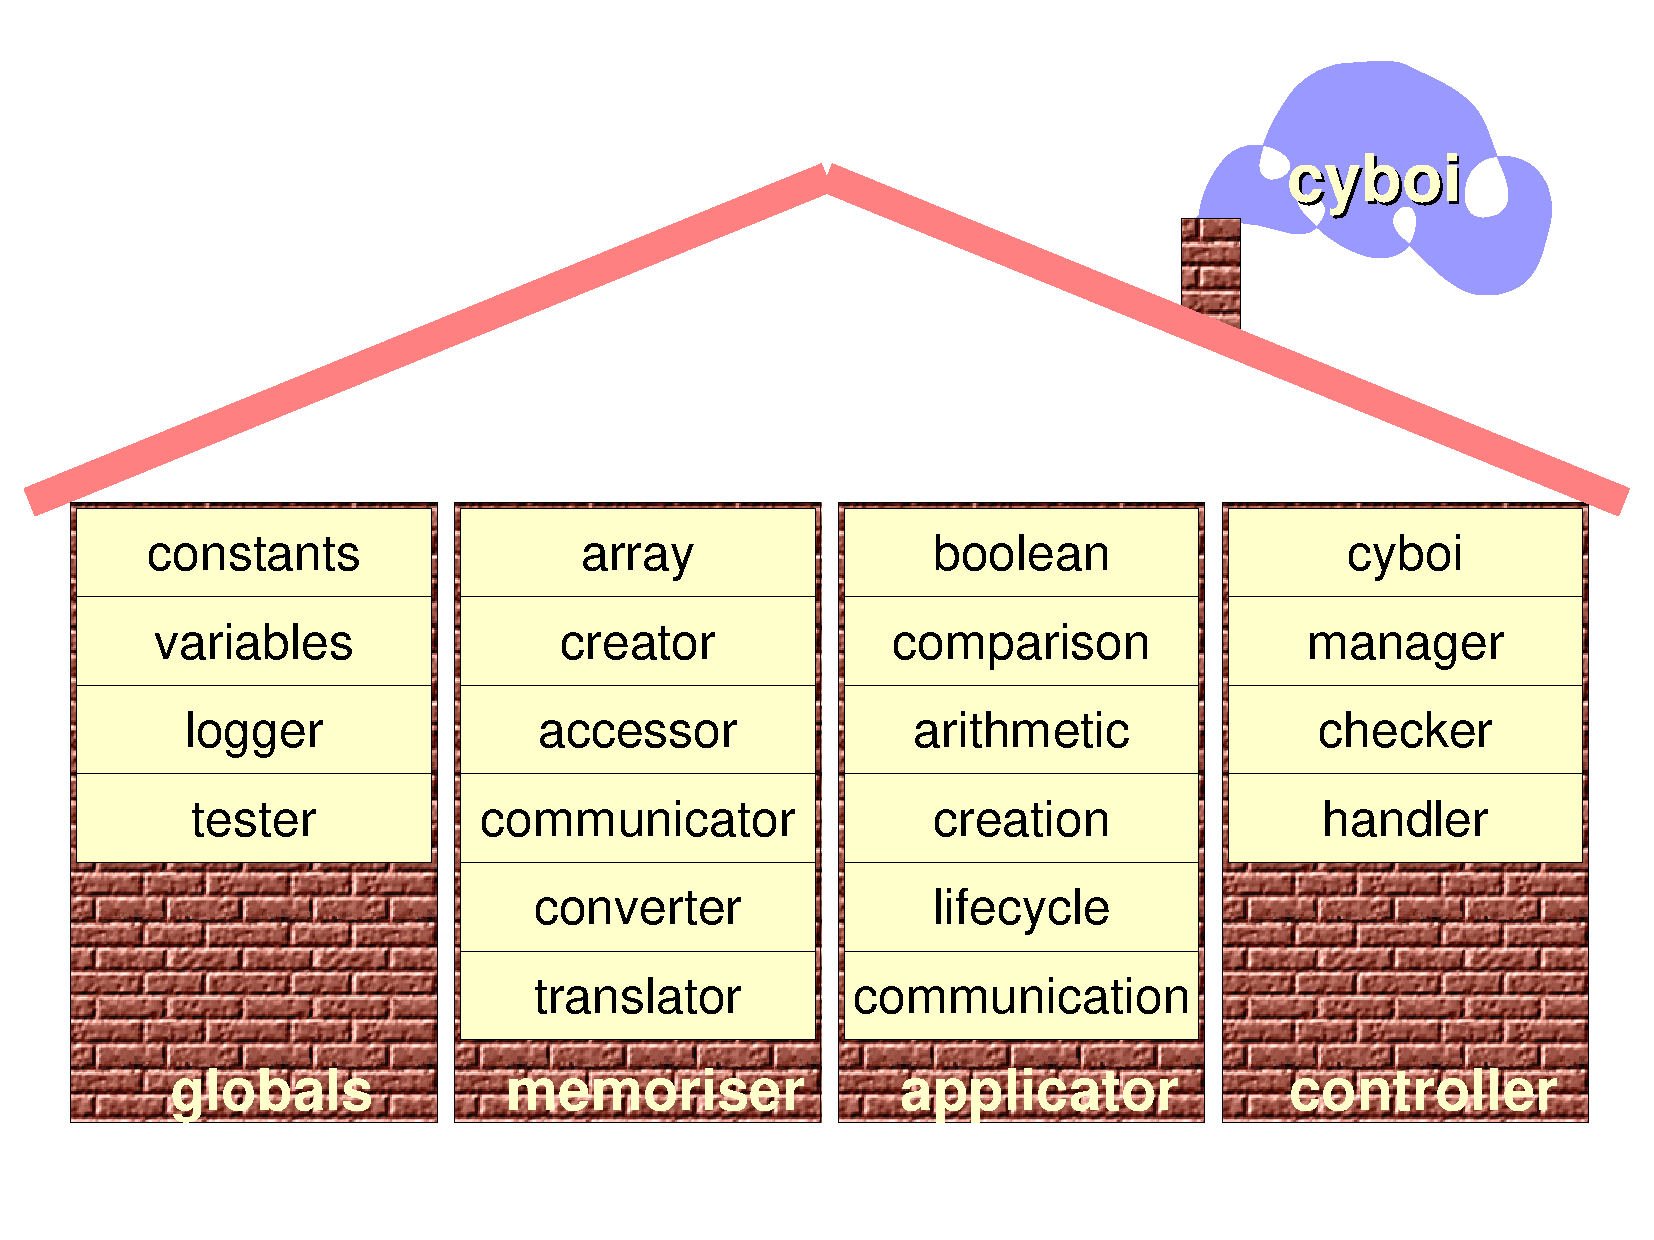
\includegraphics[scale=0.3,angle=-90]{graphic/architecture.pdf}
        \caption{CYBOI Architecture consisting of Four Parts}
        \label{architecture_figure}
    \end{center}
\end{figure}

The i/o data handling is not separated out here (as opposed to von Neumann's
model); it is managed by the controller modules. The i/o data themselves,
representing states, are stored in memory. Global constants and variables are
necessary additions. More details on the modules' functionality are given in
section \ref{functionality_in_detail_heading}.
